% Options for packages loaded elsewhere
\PassOptionsToPackage{unicode}{hyperref}
\PassOptionsToPackage{hyphens}{url}
\documentclass[
]{article}
\usepackage{xcolor}
\usepackage[margin=2.54cm]{geometry}
\usepackage{amsmath,amssymb}
\setcounter{secnumdepth}{-\maxdimen} % remove section numbering
\usepackage{iftex}
\ifPDFTeX
  \usepackage[T1]{fontenc}
  \usepackage[utf8]{inputenc}
  \usepackage{textcomp} % provide euro and other symbols
\else % if luatex or xetex
  \usepackage{unicode-math} % this also loads fontspec
  \defaultfontfeatures{Scale=MatchLowercase}
  \defaultfontfeatures[\rmfamily]{Ligatures=TeX,Scale=1}
\fi
\usepackage{lmodern}
\ifPDFTeX\else
  % xetex/luatex font selection
\fi
% Use upquote if available, for straight quotes in verbatim environments
\IfFileExists{upquote.sty}{\usepackage{upquote}}{}
\IfFileExists{microtype.sty}{% use microtype if available
  \usepackage[]{microtype}
  \UseMicrotypeSet[protrusion]{basicmath} % disable protrusion for tt fonts
}{}
\makeatletter
\@ifundefined{KOMAClassName}{% if non-KOMA class
  \IfFileExists{parskip.sty}{%
    \usepackage{parskip}
  }{% else
    \setlength{\parindent}{0pt}
    \setlength{\parskip}{6pt plus 2pt minus 1pt}}
}{% if KOMA class
  \KOMAoptions{parskip=half}}
\makeatother
\usepackage{color}
\usepackage{fancyvrb}
\newcommand{\VerbBar}{|}
\newcommand{\VERB}{\Verb[commandchars=\\\{\}]}
\DefineVerbatimEnvironment{Highlighting}{Verbatim}{commandchars=\\\{\}}
% Add ',fontsize=\small' for more characters per line
\usepackage{framed}
\definecolor{shadecolor}{RGB}{248,248,248}
\newenvironment{Shaded}{\begin{snugshade}}{\end{snugshade}}
\newcommand{\AlertTok}[1]{\textcolor[rgb]{0.94,0.16,0.16}{#1}}
\newcommand{\AnnotationTok}[1]{\textcolor[rgb]{0.56,0.35,0.01}{\textbf{\textit{#1}}}}
\newcommand{\AttributeTok}[1]{\textcolor[rgb]{0.13,0.29,0.53}{#1}}
\newcommand{\BaseNTok}[1]{\textcolor[rgb]{0.00,0.00,0.81}{#1}}
\newcommand{\BuiltInTok}[1]{#1}
\newcommand{\CharTok}[1]{\textcolor[rgb]{0.31,0.60,0.02}{#1}}
\newcommand{\CommentTok}[1]{\textcolor[rgb]{0.56,0.35,0.01}{\textit{#1}}}
\newcommand{\CommentVarTok}[1]{\textcolor[rgb]{0.56,0.35,0.01}{\textbf{\textit{#1}}}}
\newcommand{\ConstantTok}[1]{\textcolor[rgb]{0.56,0.35,0.01}{#1}}
\newcommand{\ControlFlowTok}[1]{\textcolor[rgb]{0.13,0.29,0.53}{\textbf{#1}}}
\newcommand{\DataTypeTok}[1]{\textcolor[rgb]{0.13,0.29,0.53}{#1}}
\newcommand{\DecValTok}[1]{\textcolor[rgb]{0.00,0.00,0.81}{#1}}
\newcommand{\DocumentationTok}[1]{\textcolor[rgb]{0.56,0.35,0.01}{\textbf{\textit{#1}}}}
\newcommand{\ErrorTok}[1]{\textcolor[rgb]{0.64,0.00,0.00}{\textbf{#1}}}
\newcommand{\ExtensionTok}[1]{#1}
\newcommand{\FloatTok}[1]{\textcolor[rgb]{0.00,0.00,0.81}{#1}}
\newcommand{\FunctionTok}[1]{\textcolor[rgb]{0.13,0.29,0.53}{\textbf{#1}}}
\newcommand{\ImportTok}[1]{#1}
\newcommand{\InformationTok}[1]{\textcolor[rgb]{0.56,0.35,0.01}{\textbf{\textit{#1}}}}
\newcommand{\KeywordTok}[1]{\textcolor[rgb]{0.13,0.29,0.53}{\textbf{#1}}}
\newcommand{\NormalTok}[1]{#1}
\newcommand{\OperatorTok}[1]{\textcolor[rgb]{0.81,0.36,0.00}{\textbf{#1}}}
\newcommand{\OtherTok}[1]{\textcolor[rgb]{0.56,0.35,0.01}{#1}}
\newcommand{\PreprocessorTok}[1]{\textcolor[rgb]{0.56,0.35,0.01}{\textit{#1}}}
\newcommand{\RegionMarkerTok}[1]{#1}
\newcommand{\SpecialCharTok}[1]{\textcolor[rgb]{0.81,0.36,0.00}{\textbf{#1}}}
\newcommand{\SpecialStringTok}[1]{\textcolor[rgb]{0.31,0.60,0.02}{#1}}
\newcommand{\StringTok}[1]{\textcolor[rgb]{0.31,0.60,0.02}{#1}}
\newcommand{\VariableTok}[1]{\textcolor[rgb]{0.00,0.00,0.00}{#1}}
\newcommand{\VerbatimStringTok}[1]{\textcolor[rgb]{0.31,0.60,0.02}{#1}}
\newcommand{\WarningTok}[1]{\textcolor[rgb]{0.56,0.35,0.01}{\textbf{\textit{#1}}}}
\usepackage{graphicx}
\makeatletter
\newsavebox\pandoc@box
\newcommand*\pandocbounded[1]{% scales image to fit in text height/width
  \sbox\pandoc@box{#1}%
  \Gscale@div\@tempa{\textheight}{\dimexpr\ht\pandoc@box+\dp\pandoc@box\relax}%
  \Gscale@div\@tempb{\linewidth}{\wd\pandoc@box}%
  \ifdim\@tempb\p@<\@tempa\p@\let\@tempa\@tempb\fi% select the smaller of both
  \ifdim\@tempa\p@<\p@\scalebox{\@tempa}{\usebox\pandoc@box}%
  \else\usebox{\pandoc@box}%
  \fi%
}
% Set default figure placement to htbp
\def\fps@figure{htbp}
\makeatother
\setlength{\emergencystretch}{3em} % prevent overfull lines
\providecommand{\tightlist}{%
  \setlength{\itemsep}{0pt}\setlength{\parskip}{0pt}}
\usepackage{bookmark}
\IfFileExists{xurl.sty}{\usepackage{xurl}}{} % add URL line breaks if available
\urlstyle{same}
\hypersetup{
  pdftitle={Assignment 3: Data Exploration},
  pdfauthor={Lex Clay},
  hidelinks,
  pdfcreator={LaTeX via pandoc}}

\title{Assignment 3: Data Exploration}
\author{Lex Clay}
\date{Spring 2026}

\begin{document}
\maketitle

\subsection{OVERVIEW}\label{overview}

This exercise accompanies the lessons in Environmental Data Analytics on
Data Exploration.

\subsection{Directions}\label{directions}

\begin{enumerate}
\def\labelenumi{\arabic{enumi}.}
\item
  Rename this file
  \texttt{\textless{}FirstLast\textgreater{}\_A03\_DataExploration.Rmd}
  (replacing \texttt{\textless{}FirstLast\textgreater{}} with your first
  and last name).
\item
  Change ``Student Name'' on line 3 (above) with your name.
\item
  Work through the steps, \textbf{creating code and output} that fulfill
  each instruction.
\item
  {[}NEW{]} Assign a useful \textbf{name to each code chunk} and include
  ample \textbf{comments} with your code.
\item
  Be sure to \textbf{answer the questions} in this assignment document.
\item
  When you have completed the assignment, \textbf{Knit} the text and
  code into a single PDF file.
\item
  After Knitting, submit the completed exercise (PDF file) to Canvas.
\item
  Initial here to acknowledge that you did not use AI in completing this
  assignment, except where expressly allowed: \_\_\_
\end{enumerate}

\textbf{TIP}: If your code extends past the page when knit, tidy your
code by manually inserting line breaks in your code chunks.

\textbf{TIP}: If your code fails to knit, check: * That no
\texttt{install.packages()} or \texttt{View()} commands exist in your
code. * That you are not displaying the entire contents of a large
dataframe in your code.

\begin{center}\rule{0.5\linewidth}{0.5pt}\end{center}

\subsection{Set up your R session}\label{set-up-your-r-session}

\begin{enumerate}
\def\labelenumi{\arabic{enumi}.}
\tightlist
\item
  Load necessary packages (tidyverse, here), check your current working
  directory and import two datasets: the ECOTOX neonicotinoid dataset
  (ECOTOX\_Neonicotinoids\_Insects\_raw.csv) and the Niwot Ridge NEON
  dataset for litter and woody debris
  (NEON\_NIWO\_Litter\_massdata\_2018-08\_raw.csv). Name these datasets
  ``Neonics'' and ``Litter'', respectively.
\end{enumerate}

\textbf{Be sure to}: * Use the \texttt{here()} package in specifying the
paths to your datasets * Include the appropriate subcommand to read in
character based columns as factors

\begin{Shaded}
\begin{Highlighting}[]
\CommentTok{\#Here I load libraries and CSV files}

\FunctionTok{library}\NormalTok{(tidyverse)}
\FunctionTok{library}\NormalTok{(here)}
\end{Highlighting}
\end{Shaded}

\begin{verbatim}
## Warning: package 'here' was built under R version 4.5.2
\end{verbatim}

\begin{Shaded}
\begin{Highlighting}[]
\FunctionTok{getwd}\NormalTok{()}
\end{Highlighting}
\end{Shaded}

\begin{verbatim}
## [1] "C:/Users/lexcl/OneDrive/Documents/EDE/EDE_Spring2026"
\end{verbatim}

\begin{Shaded}
\begin{Highlighting}[]
\FunctionTok{here}\NormalTok{()}
\end{Highlighting}
\end{Shaded}

\begin{verbatim}
## [1] "C:/Users/lexcl/OneDrive/Documents/EDE/EDE_Spring2026"
\end{verbatim}

\begin{Shaded}
\begin{Highlighting}[]
\NormalTok{Neonics }\OtherTok{\textless{}{-}} \FunctionTok{read.csv}\NormalTok{(}\AttributeTok{file=}\FunctionTok{here}\NormalTok{(}\StringTok{"./Data/Raw/ECOTOX\_Neonicotinoids\_Insects\_raw.csv"}\NormalTok{),}\AttributeTok{stringsAsFactors =}\ConstantTok{TRUE}\NormalTok{)}

\NormalTok{Litter }\OtherTok{\textless{}{-}} \FunctionTok{read.csv}\NormalTok{(}\AttributeTok{file=}\FunctionTok{here}\NormalTok{(}\StringTok{"./Data/Raw/NIWO\_Litter/NEON\_NIWO\_Litter\_massdata\_2018{-}08\_raw.csv"}\NormalTok{),}\AttributeTok{stringsAsFactors =} \ConstantTok{TRUE}\NormalTok{)}
\end{Highlighting}
\end{Shaded}

\subsection{Learn about your system}\label{learn-about-your-system}

\begin{enumerate}
\def\labelenumi{\arabic{enumi}.}
\setcounter{enumi}{1}
\tightlist
\item
  The neonicotinoid dataset was collected from the Environmental
  Protection Agency's ECOTOX Knowledgebase, a database for ecotoxicology
  research. Neonicotinoids are a class of insecticides used widely in
  agriculture. The dataset that has been pulled includes all studies
  published on insects. Why might we be interested in the ecotoxicology
  of neonicotinoids on insects? Feel free to do a brief internet search
  if you feel you need more background information. (AI is allowed here,
  but put answers in your own words.)
\end{enumerate}

\begin{quote}
Answer:
\end{quote}

My guess is that the effects of pesticides observed on insects might
serve as indicators of potential effects on other species, and/or the
well-being of the ecosystem they inhabit. We might also be able to
discern whether insects are developing resistance to the pesticides
presumably designed to kill them.

\begin{enumerate}
\def\labelenumi{\arabic{enumi}.}
\setcounter{enumi}{2}
\tightlist
\item
  The Niwot Ridge litter and woody debris dataset was collected from the
  National Ecological Observatory Network, which collectively includes
  81 aquatic and terrestrial sites across 20 ecoclimatic domains. 32 of
  these sites sample forest litter and woody debris, and we will focus
  on the Niwot Ridge long-term ecological research (LTER) station in
  Colorado. Why might we be interested in studying litter and woody
  debris that falls to the ground in forests? Feel free to do a brief
  internet search if you feel you need more background information. (AI
  is allowed here, but put answers in your own words.)
\end{enumerate}

\begin{quote}
Answer:
\end{quote}

Another guess here. If looking at the food people eat can help us
understand a human's general health, examining litter and woody debris
might help us gain insights into the health of the forest ground/soil.
Such debris is also consumed by many species, including termites and
other insects with an insatiable hankering for wood.

Maybe I am speculating now about how these two data sites are related,
but it is many of these debris-eating species that are targeted by
insecticides, potentially disrupting natural processes of
decomposition/the nutrient cycle.

\begin{enumerate}
\def\labelenumi{\arabic{enumi}.}
\setcounter{enumi}{3}
\tightlist
\item
  How is litter and woody debris sampled as part of the NEON network?
  Read the NEON\_Litterfall\_UserGuide.pdf document to learn more. List
  three pieces of salient information about the sampling methods here:
\end{enumerate}

\begin{quote}
Answer: 1.Litter and fine woody debris samplig is taken only at sites
with vegetation \textgreater{} 2m tall and only in tower plots(page 3.)
2.In sites with \textgreater50\% cover of woody vegetation, placement of
litter traps is random.In sites with \textless50\% cover, litter traps
are placed in areas beneath the qualifying vegetation measure. 3.Sample
data is nested in the following structure: subplotID \textless{} plotID
\textless{} siteID \textless{} domainID.
\end{quote}

\subsection{Obtain basic summaries of your data
(Neonics)}\label{obtain-basic-summaries-of-your-data-neonics}

\begin{enumerate}
\def\labelenumi{\arabic{enumi}.}
\setcounter{enumi}{4}
\tightlist
\item
  What are the dimensions of the dataset?
\end{enumerate}

\begin{Shaded}
\begin{Highlighting}[]
\FunctionTok{dim}\NormalTok{(Neonics)}
\end{Highlighting}
\end{Shaded}

\begin{verbatim}
## [1] 4623   30
\end{verbatim}

\begin{Shaded}
\begin{Highlighting}[]
\CommentTok{\#answer: dimensions are 4623    30 }
\end{Highlighting}
\end{Shaded}

\begin{enumerate}
\def\labelenumi{\arabic{enumi}.}
\setcounter{enumi}{5}
\tightlist
\item
  Using the \texttt{summary} function on the ``Effect'' column,
  determine the most common effects that are studied. {[}Tip: The
  \texttt{sort()} command is useful for listing the values in order of
  magnitude\ldots{]}
\end{enumerate}

\begin{Shaded}
\begin{Highlighting}[]
\CommentTok{\#}
\FunctionTok{summary}\NormalTok{(Neonics}\SpecialCharTok{$}\NormalTok{Effect)}\SpecialCharTok{\%\textgreater{}\%}\FunctionTok{sort}\NormalTok{()}
\end{Highlighting}
\end{Shaded}

\begin{verbatim}
##       Hormone(s)        Histology       Physiology          Cell(s) 
##                1                5                7                9 
##     Biochemistry     Accumulation     Intoxication    Immunological 
##               11               12               12               16 
##       Morphology           Growth        Enzyme(s)         Genetics 
##               22               38               62               82 
##        Avoidance      Development     Reproduction Feeding behavior 
##              102              136              197              255 
##         Behavior        Mortality       Population 
##              360             1493             1803
\end{verbatim}

Question: Which two effects stand out as the most studied? Can you guess
why these effects might specifically be of interest? \textgreater{}
Answer: Mortality and Population stand out as the most studied
presumably because they are the most closely associated with a species'
survival.

\begin{enumerate}
\def\labelenumi{\arabic{enumi}.}
\setcounter{enumi}{6}
\tightlist
\item
  Using the \texttt{summary} function, determine the six most commonly
  studied species in the dataset (common name).{[}TIP: Explore the help
  on the \texttt{summary()} function, in particular the \texttt{maxsum}
  argument\ldots{]}
\end{enumerate}

\begin{Shaded}
\begin{Highlighting}[]
\FunctionTok{summary}\NormalTok{(Neonics}\SpecialCharTok{$}\NormalTok{Species.Group, }\AttributeTok{maxsum =}\DecValTok{6}\NormalTok{)}
\end{Highlighting}
\end{Shaded}

\begin{verbatim}
##                                               Insects/Spiders 
##                                                          3569 
##                        Insects/Spiders; Standard Test Species 
##                                                            27 
## Insects/Spiders; Standard Test Species; U.S. Invasive Species 
##                                                           667 
##                        Insects/Spiders; U.S. Invasive Species 
##                                                           360
\end{verbatim}

\begin{Shaded}
\begin{Highlighting}[]
\FunctionTok{summary}\NormalTok{(Neonics}\SpecialCharTok{$}\NormalTok{Species.Common.Name, }\AttributeTok{maxsum =}\DecValTok{6}\NormalTok{)}
\end{Highlighting}
\end{Shaded}

\begin{verbatim}
##             Honey Bee        Parasitic Wasp Buff Tailed Bumblebee 
##                   667                   285                   183 
##   Carniolan Honey Bee            Bumble Bee               (Other) 
##                   152                   140                  3196
\end{verbatim}

\begin{Shaded}
\begin{Highlighting}[]
\FunctionTok{summary}\NormalTok{(Neonics}\SpecialCharTok{$}\NormalTok{Test.Location, }\AttributeTok{maxsum =}\DecValTok{6}\NormalTok{)}
\end{Highlighting}
\end{Shaded}

\begin{verbatim}
##     Field artificial        Field natural Field undeterminable 
##                   96                 1663                    4 
##                  Lab 
##                 2860
\end{verbatim}

► Question: What do these species have in common? Why might they be of
interest over other insects? \textgreater{} Answer: With the exception
of the (other) group, they are all species of bees.Their role as
pollinators makes them important.

\begin{enumerate}
\def\labelenumi{\arabic{enumi}.}
\setcounter{enumi}{7}
\tightlist
\item
  The \texttt{Conc.1..Author} column, which lists the concentration of
  the neonicitoid dose, should include numeric values. What is the class
  of \texttt{Conc.1..Author.} column in the dataset, and why is it not
  numeric? {[}Tip: Viewing the dataframe may be helpful\ldots{]}
\end{enumerate}

\begin{Shaded}
\begin{Highlighting}[]
\FunctionTok{class}\NormalTok{(}\StringTok{"Conc.1..Author"}\NormalTok{)}
\end{Highlighting}
\end{Shaded}

\begin{verbatim}
## [1] "character"
\end{verbatim}

\begin{Shaded}
\begin{Highlighting}[]
\FunctionTok{View}\NormalTok{(Neonics)}
\end{Highlighting}
\end{Shaded}

\begin{quote}
Answer: \#Conc.1..Author is categorized as a character instead of
numeric because the column (which is a vector) can only store data
points from one data type. Since some entries list ``NR'' instead of a
numeric concentration, it was classified as a character.
\end{quote}

\subsection{Explore your data graphically
(Neonics)}\label{explore-your-data-graphically-neonics}

\begin{enumerate}
\def\labelenumi{\arabic{enumi}.}
\setcounter{enumi}{8}
\tightlist
\item
  Using \texttt{geom\_freqpoly}, generate a plot of the number of
  studies conducted by publication year.
\end{enumerate}

\begin{Shaded}
\begin{Highlighting}[]
\FunctionTok{ggplot}\NormalTok{(Neonics) }\SpecialCharTok{+}
  \FunctionTok{geom\_freqpoly}\NormalTok{(}\FunctionTok{aes}\NormalTok{(}\AttributeTok{x =}\NormalTok{ Publication.Year))}
\end{Highlighting}
\end{Shaded}

\begin{verbatim}
## `stat_bin()` using `bins = 30`. Pick better value `binwidth`.
\end{verbatim}

\pandocbounded{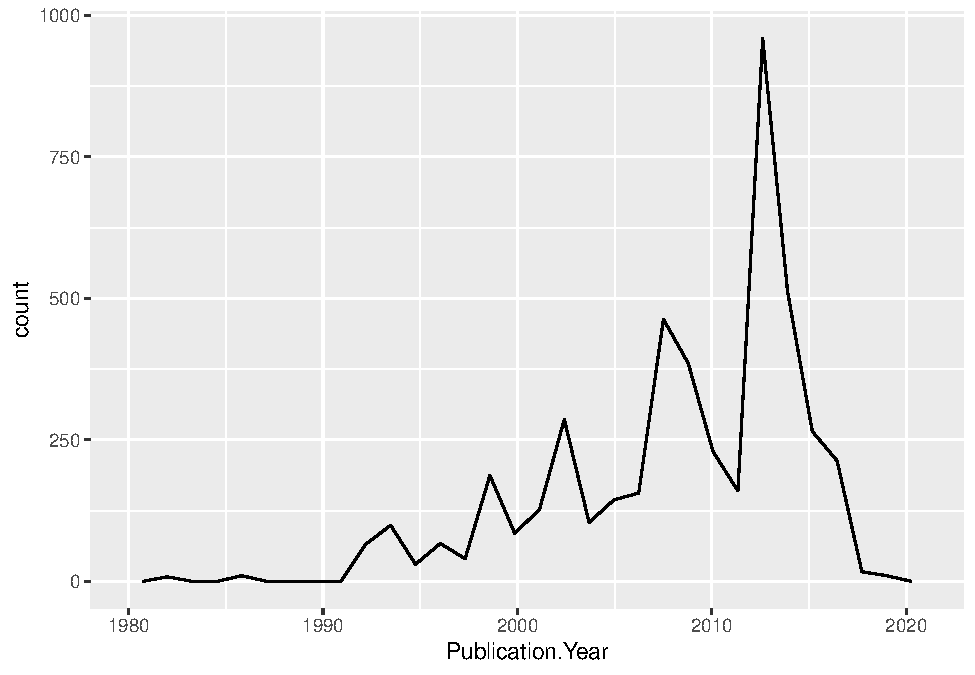
\includegraphics[keepaspectratio]{LexClayA03_DataExploration_files/figure-latex/Studies by Pub Year-1.pdf}}

\begin{enumerate}
\def\labelenumi{\arabic{enumi}.}
\setcounter{enumi}{9}
\tightlist
\item
  Reproduce the same graph but now add a color aesthetic so that
  different Test.Location are displayed as different colors.
\end{enumerate}

\begin{Shaded}
\begin{Highlighting}[]
\FunctionTok{ggplot}\NormalTok{(Neonics)}\SpecialCharTok{+} 
  \FunctionTok{geom\_freqpoly}\NormalTok{(}\FunctionTok{aes}\NormalTok{(}\AttributeTok{x =}\NormalTok{ Publication.Year, }\AttributeTok{color=}\NormalTok{Test.Location))}
\end{Highlighting}
\end{Shaded}

\begin{verbatim}
## `stat_bin()` using `bins = 30`. Pick better value `binwidth`.
\end{verbatim}

\pandocbounded{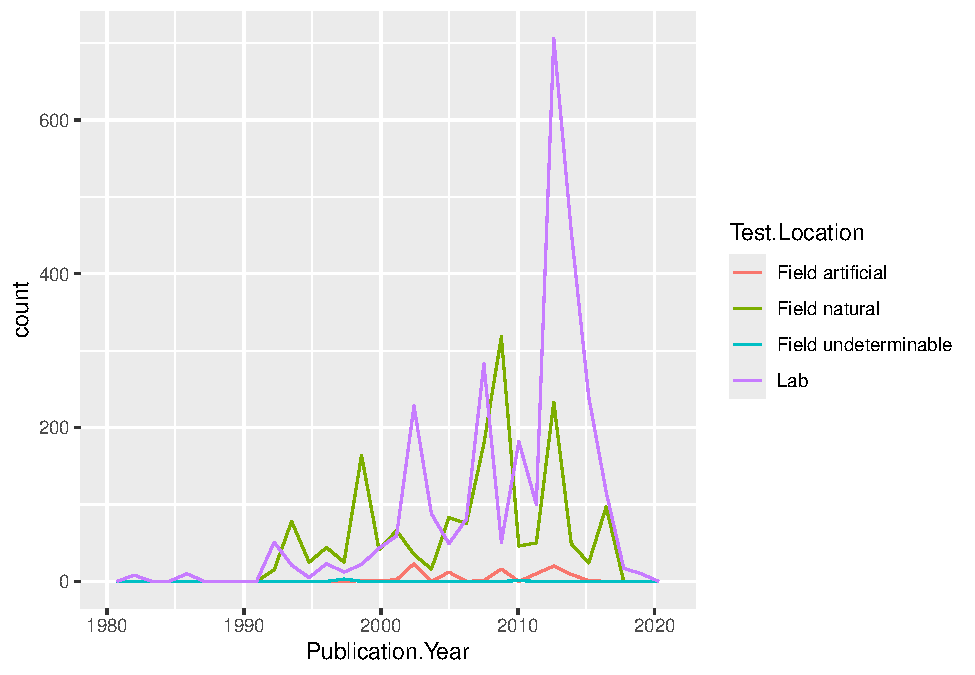
\includegraphics[keepaspectratio]{LexClayA03_DataExploration_files/figure-latex/Studies by Pub Year by Location-1.pdf}}

►Interpret this graph. What are the most common test locations, and do
they differ over time? \textgreater{} Answer: Field natural is the most
common test location for a period right before 2010. Overall, Lab is the
most common test location with a significant uptick between 2010 and
2020.

\begin{enumerate}
\def\labelenumi{\arabic{enumi}.}
\setcounter{enumi}{10}
\tightlist
\item
  Create a bar graph of Endpoint counts.
\end{enumerate}

{[}\textbf{TIP}: Add
\texttt{theme(axis.text.x\ =\ element\_text(angle\ =\ 90,\ vjust\ =\ 0.5,\ hjust=1))}
to the end of your plot command to rotate and align the X-axis
labels\ldots{]}

\begin{Shaded}
\begin{Highlighting}[]
\FunctionTok{ggplot}\NormalTok{(}\AttributeTok{data=}\NormalTok{Neonics, }\FunctionTok{aes}\NormalTok{(}\AttributeTok{x=}\NormalTok{ Endpoint))}\SpecialCharTok{+}\FunctionTok{theme}\NormalTok{(}\AttributeTok{axis.text.x =} \FunctionTok{element\_text}\NormalTok{(}\AttributeTok{angle =} \DecValTok{90}\NormalTok{, }\AttributeTok{vjust =} \FloatTok{0.5}\NormalTok{, }\AttributeTok{hjust=}\DecValTok{1}\NormalTok{))}\SpecialCharTok{+}
  \FunctionTok{geom\_bar}\NormalTok{(}\AttributeTok{fill =}\StringTok{"\#5C4033"}\NormalTok{) }
\end{Highlighting}
\end{Shaded}

\pandocbounded{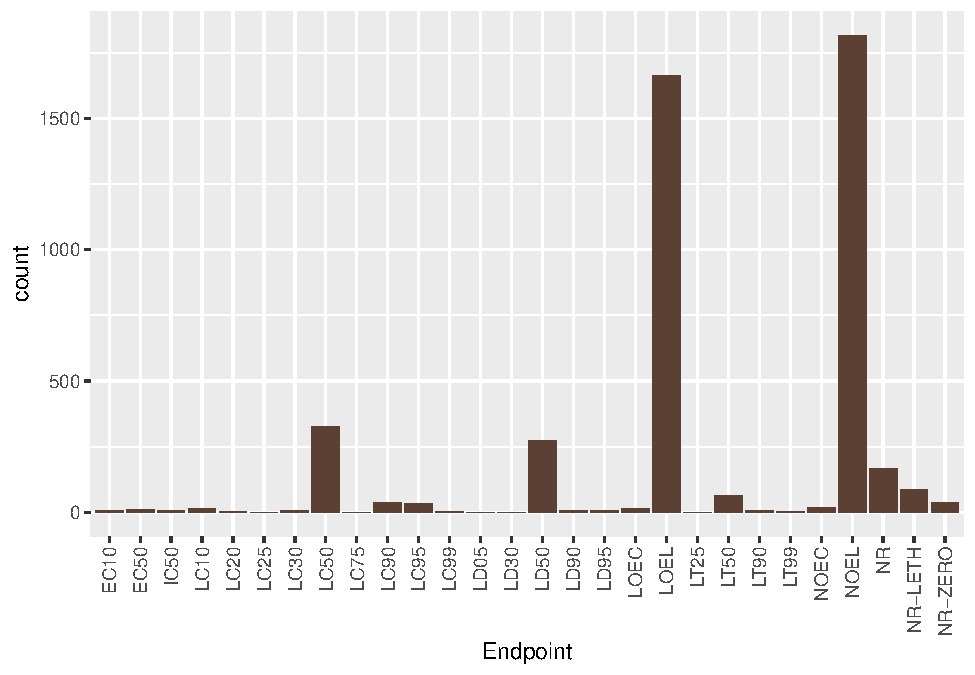
\includegraphics[keepaspectratio]{LexClayA03_DataExploration_files/figure-latex/Endpoint Counts-1.pdf}}

► What are the two most common end points, and how are they defined?
Consult the ECOTOX\_CodeAppendix (p.721) for more information.
\textgreater{} Answer: The two most common end points are LOEL(lowest
observable effect level) and NOEL(no observable effect level.) Both
measure the effect relative to controls. ---

\subsection{Explore your data (Litter)}\label{explore-your-data-litter}

\begin{enumerate}
\def\labelenumi{\arabic{enumi}.}
\setcounter{enumi}{11}
\tightlist
\item
  Determine the class of \texttt{collectDate}. Is it a date? If not,
  change to a date and confirm the new class of the variable. Using the
  \texttt{unique} function, determine which dates litter was sampled in
  August 2018.
\end{enumerate}

\begin{Shaded}
\begin{Highlighting}[]
\FunctionTok{class}\NormalTok{(}\StringTok{"collectDate"}\NormalTok{)}\CommentTok{\#shows that it is a character not a date }
\end{Highlighting}
\end{Shaded}

\begin{verbatim}
## [1] "character"
\end{verbatim}

\begin{Shaded}
\begin{Highlighting}[]
\NormalTok{Litter}\SpecialCharTok{$}\NormalTok{collectDate }\OtherTok{\textless{}{-}}\FunctionTok{as.Date}\NormalTok{(Litter}\SpecialCharTok{$}\NormalTok{collectDate, }\AttributeTok{format=}\StringTok{\textquotesingle{}\%Y{-}\%m{-}\%d\textquotesingle{}}\NormalTok{)}

\FunctionTok{class}\NormalTok{(Litter}\SpecialCharTok{$}\NormalTok{collectDate) }\CommentTok{\#confirmed it is a date now }
\end{Highlighting}
\end{Shaded}

\begin{verbatim}
## [1] "Date"
\end{verbatim}

\begin{enumerate}
\def\labelenumi{\arabic{enumi}.}
\setcounter{enumi}{12}
\tightlist
\item
  Using the \texttt{unique} function, list the different
  \texttt{plotIDs} sampled at Niwot Ridge.
\end{enumerate}

\begin{Shaded}
\begin{Highlighting}[]
\FunctionTok{unique}\NormalTok{(Litter}\SpecialCharTok{$}\NormalTok{plotID)}
\end{Highlighting}
\end{Shaded}

\begin{verbatim}
##  [1] NIWO_061 NIWO_064 NIWO_067 NIWO_040 NIWO_041 NIWO_063 NIWO_047 NIWO_051
##  [9] NIWO_058 NIWO_046 NIWO_062 NIWO_057
## 12 Levels: NIWO_040 NIWO_041 NIWO_046 NIWO_047 NIWO_051 NIWO_057 ... NIWO_067
\end{verbatim}

\begin{Shaded}
\begin{Highlighting}[]
\FunctionTok{summary}\NormalTok{(Litter}\SpecialCharTok{$}\NormalTok{plotID)}
\end{Highlighting}
\end{Shaded}

\begin{verbatim}
## NIWO_040 NIWO_041 NIWO_046 NIWO_047 NIWO_051 NIWO_057 NIWO_058 NIWO_061 
##       20       19       18       15       14        8       16       17 
## NIWO_062 NIWO_063 NIWO_064 NIWO_067 
##       14       14       16       17
\end{verbatim}

\begin{Shaded}
\begin{Highlighting}[]
\FunctionTok{class}\NormalTok{(Litter}\SpecialCharTok{$}\NormalTok{plotID) }\CommentTok{\#this is a factor }
\end{Highlighting}
\end{Shaded}

\begin{verbatim}
## [1] "factor"
\end{verbatim}

► How is the information obtained from \texttt{unique} different from
that obtained from \texttt{summary}? \textgreater{} Answer:The unique
function simply lists the unique IDs without duplicates. The summary
function includes the number of times each unique ID appears in the data
set.

\begin{enumerate}
\def\labelenumi{\arabic{enumi}.}
\setcounter{enumi}{13}
\tightlist
\item
  Create a bar graph of \texttt{functionalGroup} counts. This shows you
  what type of litter is collected at the Niwot Ridge sites. Notice that
  litter types are fairly equally distributed across the Niwot Ridge
  sites.
\end{enumerate}

\begin{Shaded}
\begin{Highlighting}[]
\FunctionTok{ggplot}\NormalTok{(}\AttributeTok{data=}\NormalTok{Litter, }\FunctionTok{aes}\NormalTok{(}\AttributeTok{x =}\NormalTok{functionalGroup))}\SpecialCharTok{+}
  \FunctionTok{geom\_bar}\NormalTok{()}
\end{Highlighting}
\end{Shaded}

\pandocbounded{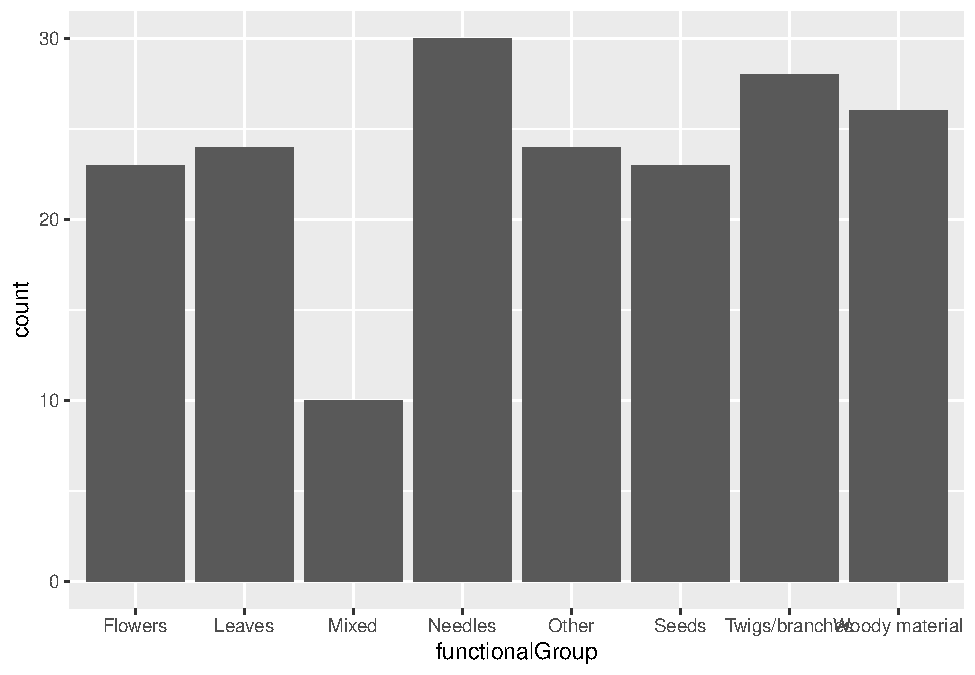
\includegraphics[keepaspectratio]{LexClayA03_DataExploration_files/figure-latex/functionalGroup Counts-1.pdf}}

\begin{enumerate}
\def\labelenumi{\arabic{enumi}.}
\setcounter{enumi}{14}
\tightlist
\item
  Using \texttt{geom\_boxplot} and \texttt{geom\_violin}, create a
  boxplot and a violin plot of \texttt{dryMass} by
  \texttt{functionalGroup}.
\end{enumerate}

\begin{Shaded}
\begin{Highlighting}[]
\FunctionTok{ggplot}\NormalTok{(Litter)}\SpecialCharTok{+}
  \FunctionTok{geom\_boxplot}\NormalTok{(}\FunctionTok{aes}\NormalTok{(}\AttributeTok{x =}\NormalTok{ functionalGroup, }\AttributeTok{y =}\NormalTok{ dryMass))}
\end{Highlighting}
\end{Shaded}

\pandocbounded{\includegraphics[keepaspectratio]{LexClayA03_DataExploration_files/figure-latex/Boxplot v. Violin plot: Which shows this data best?-1.pdf}}

\begin{Shaded}
\begin{Highlighting}[]
\FunctionTok{ggplot}\NormalTok{(Litter)}\SpecialCharTok{+}
  \FunctionTok{geom\_violin}\NormalTok{(}\FunctionTok{aes}\NormalTok{(}\AttributeTok{x=}\NormalTok{functionalGroup, }\AttributeTok{y=}\NormalTok{dryMass))}
\end{Highlighting}
\end{Shaded}

\pandocbounded{\includegraphics[keepaspectratio]{LexClayA03_DataExploration_files/figure-latex/Boxplot v. Violin plot: Which shows this data best?-2.pdf}}

► Why is the boxplot a more effective visualization option than the
violin plot in this case? \textgreater{} Answer:The box plot shows the
actual variation between the data points, whereas the violin plot
oversimplifies to a straight line.

► What type(s) of litter tend to have the highest biomass at these
sites? \textgreater{} Answer: Needles have the highest biomass, with a
median biomass of almost 2.5.

\end{document}
